% Created 2021-09-27 Mon 12:01
% Intended LaTeX compiler: xelatex
\documentclass[letterpaper]{article}
\usepackage{graphicx}
\usepackage{grffile}
\usepackage{longtable}
\usepackage{wrapfig}
\usepackage{rotating}
\usepackage[normalem]{ulem}
\usepackage{amsmath}
\usepackage{textcomp}
\usepackage{amssymb}
\usepackage{capt-of}
\usepackage{hyperref}
\setlength{\parindent}{0pt}
\usepackage[margin=1in]{geometry}
\usepackage{fontspec}
\usepackage{svg}
\usepackage{cancel}
\usepackage{indentfirst}
\setmainfont[ItalicFont = LiberationSans-Italic, BoldFont = LiberationSans-Bold, BoldItalicFont = LiberationSans-BoldItalic]{LiberationSans}
\newfontfamily\NHLight[ItalicFont = LiberationSansNarrow-Italic, BoldFont       = LiberationSansNarrow-Bold, BoldItalicFont = LiberationSansNarrow-BoldItalic]{LiberationSansNarrow}
\newcommand\textrmlf[1]{{\NHLight#1}}
\newcommand\textitlf[1]{{\NHLight\itshape#1}}
\let\textbflf\textrm
\newcommand\textulf[1]{{\NHLight\bfseries#1}}
\newcommand\textuitlf[1]{{\NHLight\bfseries\itshape#1}}
\usepackage{fancyhdr}
\pagestyle{fancy}
\usepackage{titlesec}
\usepackage{titling}
\makeatletter
\lhead{\textbf{\@title}}
\makeatother
\rhead{\textrmlf{Compiled} \today}
\lfoot{\theauthor\ \textbullet \ \textbf{2021-2022}}
\cfoot{}
\rfoot{\textrmlf{Page} \thepage}
\renewcommand{\tableofcontents}{}
\titleformat{\section} {\Large} {\textrmlf{\thesection} {|}} {0.3em} {\textbf}
\titleformat{\subsection} {\large} {\textrmlf{\thesubsection} {|}} {0.2em} {\textbf}
\titleformat{\subsubsection} {\large} {\textrmlf{\thesubsubsection} {|}} {0.1em} {\textbf}
\setlength{\parskip}{0.45em}
\renewcommand\maketitle{}
\author{Houjun Liu}
\date{\today}
\title{Viral Replication}
\hypersetup{
 pdfauthor={Houjun Liu},
 pdftitle={Viral Replication},
 pdfkeywords={},
 pdfsubject={},
 pdfcreator={Emacs 28.0.50 (Org mode 9.4.4)}, 
 pdflang={English}}
\begin{document}

\tableofcontents



\section{Viral Replication}
\label{sec:org66f3ab9}
This is the process by which the genetic material virus (and by proxy
its whole) is replicated through hijacking the host cell's
\href{KBhBIO101CentralDogma.org}{KBhBIO101CentralDogma} processes. To
investigate this, we ask two questions:

\begin{itemize}
\item \textbf{How are viral mRNAs produced from the viral genome?} => virus will
hijack the ribosomes in the host cells. So, it is more important to
ask how the mRNAs are produced to tell ribosomes what to do
\item \textbf{What serves as the template for viral genome replication} =>
replication will need a polymeraese; but the source and mechanism is
dependent on viral genome structure/composition
\end{itemize}

\subsection{For DNA Viruses}
\label{sec:org68c2b9f}
\subsubsection{How are viral mRNAs produced from the viral genome?}
\label{sec:orgd7ee65f}
\begin{itemize}
\item Viral DNA enters, through RNA polymerase II in the host cell, mRNA is
produced
\item mRNAs then read by ribosomes, and there we go
\end{itemize}

\subsubsection{What serves as the templates for viral genome replication?}
\label{sec:org519623f}
\begin{itemize}
\item Viral DNA serves as template for host cell DNA polymerase
\item Viral genome copied repeatedly
\item Virus, then, \textbf{will be replicated within the nucleus} due to it needing
the host polymerase to copy DNA
\end{itemize}

Except! Poxvirade viruses carry their own polymerase, so they replicate
in the cytoplasm by simply entering and releasing the polymerease.

\begin{figure}[htbp]
\centering
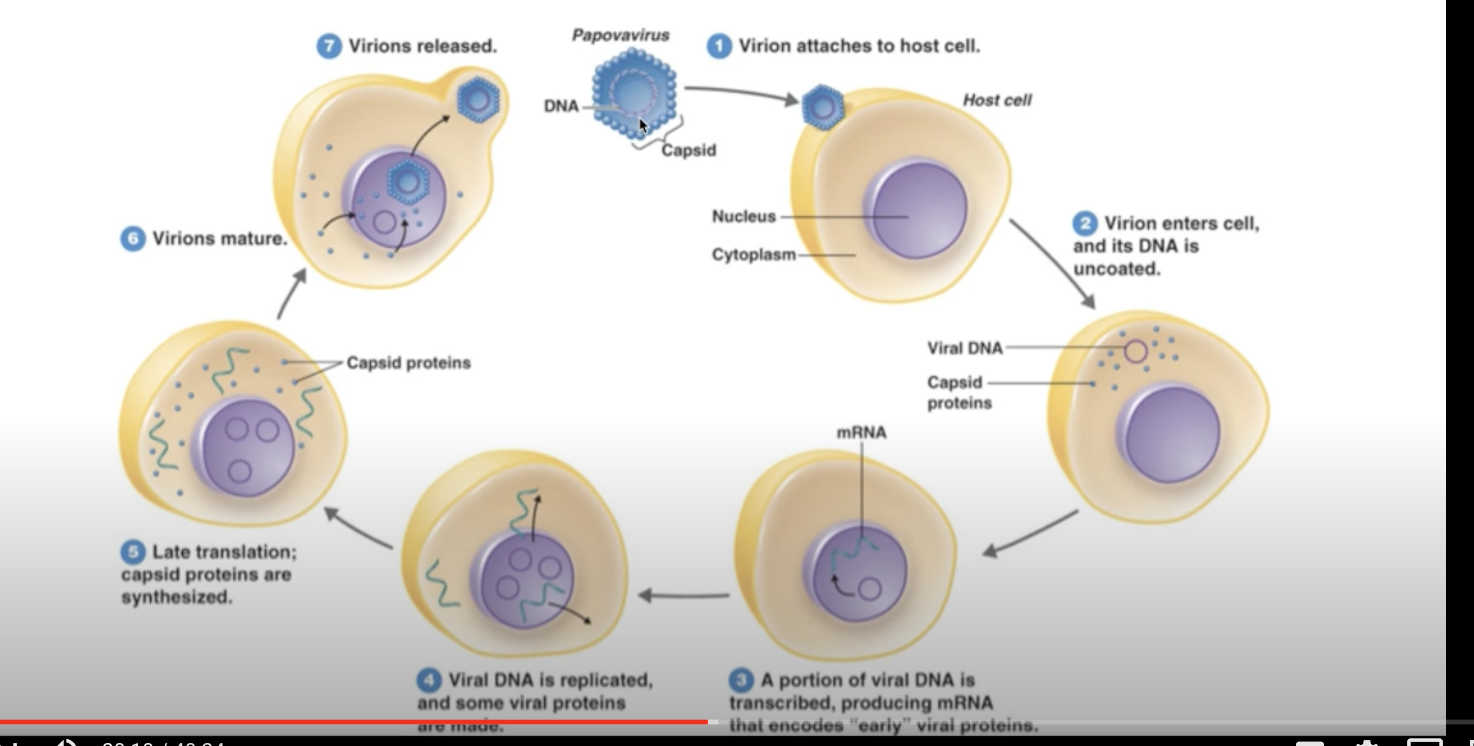
\includegraphics[width=.9\linewidth]{Screen Shot 2020-10-12 at 11.09.46 PM.png}
\caption{Screen Shot 2020-10-12 at 11.09.46 PM.png}
\end{figure}

\subsection{RNA Viruses}
\label{sec:orgab76591}
\subsubsection{How are viral mRNAs produced from the viral genome?}
\label{sec:org550a9f0}
Depends on what
\href{KBhBIO101SenseAndAntisense.org}{KBhBIO101SenseAndAntisense} the
viral RNA is, there are different processes

\begin{itemize}
\item If the virus is carrying +SS RNA, they do not need to produce anything
because that is directly translatable by the host ribosomes
\item If the virus is carrying -SS RNA (which is useless by itself as it is
the template RNA, making it harder to detect), they would trigger the
process of RNA replication either using their own RNA-dependent RNA
polymerease or using that of the host cells
\item If the virus is carrying both, it will infect with both +-stranded and
--stranded RNA, but the latter requires conversion
\end{itemize}

\subsubsection{What serves as the templates for viral genome replication?}
\label{sec:orgbb6f50c}
\begin{itemize}
\item with dsRNA; takes +ssRNA and makes -ssRMA; combining the two to
produce dsRNA
\item with +ssRNA, takes +ssRNA and makes temporary -ssRNA which makes more
+ssRNA
\item with -ssRNA, takes -ssRNA, and makes temporary +ssRNA, which makes
-ssRNA
\end{itemize}

Instead of waiting for the RNA-dependent-RNA polymerease of the cell,
viruses sometimes decide to just bring-your-own-polymerease to catalyze
this process.
\end{document}
